%!TEX TS-program = xelatex
\documentclass[]{cv}
\usepackage{afterpage}
\usepackage{hyperref}
\usepackage{color}
\usepackage{xcolor}
\usepackage{smartdiagram}
\usepackage{fontspec}
% compile the tex file with LuaLaTeX References:
%   http://texdoc.net/texmf-dist/doc/latex/fontawesome/fontawesome.pdf
%   https://www.ctan.org/tex-archive/fonts/fontawesome?lang=en
% \usepackage{fontawesome}
\usepackage[none]{hyphenat}
\usepackage{metalogo}
\usepackage{dtklogos}
\usepackage[utf8]{inputenc}
\usepackage{tikz}
\usetikzlibrary{mindmap,shadows}

\hypersetup{
    pdftitle={},
    pdfauthor={},
    pdfsubject={},
    pdfkeywords={},
    colorlinks=false,           % no link border color
    allbordercolors=white       % white border color for all
}
\smartdiagramset{
    bubble center node font = \scriptsize,
    bubble node font = \tiny,
    % specifies the minimum size of the bubble center node
    bubble center node size = 0.4cm,
    %  specifies the minimum size of the bubbles
    bubble node size = 0.4cm,
    % specifies which is the distance among the bubble center node and the other bubbles
    distance center/other bubbles = 0.3cm,
    % sets the distance from the text to the border of the bubble center node
    distance text center bubble = 0.3cm,
    % set center bubble color
    bubble center node color = materialblue,
    % define the list of colors usable in the diagram
    set color list = {materialgreen, materialred, materialcyan, green, materialorange, materialamber, materialteal, materialindigo, materiallime, materialpurple},
    % sets the opacity at which the bubbles are shown
    bubble fill opacity = 0.4,
    % sets the opacity at which the bubble text is shown
    bubble text opacity = 0.8,
}

\addbibresource{bibliography.bib}
\RequirePackage{xcolor}
\definecolor{pblue}{HTML}{0395DE}

\begin{document}
\header{Max Liao}{}
{Software Engineer}
\par
% Fake text to add separator      
\fcolorbox{white}{gray}{\parbox{\dimexpr\textwidth-2\fboxsep-2\fboxrule}{%
		.....
	}}

% In the aside, each new line forces a line break
\begin{aside}
	%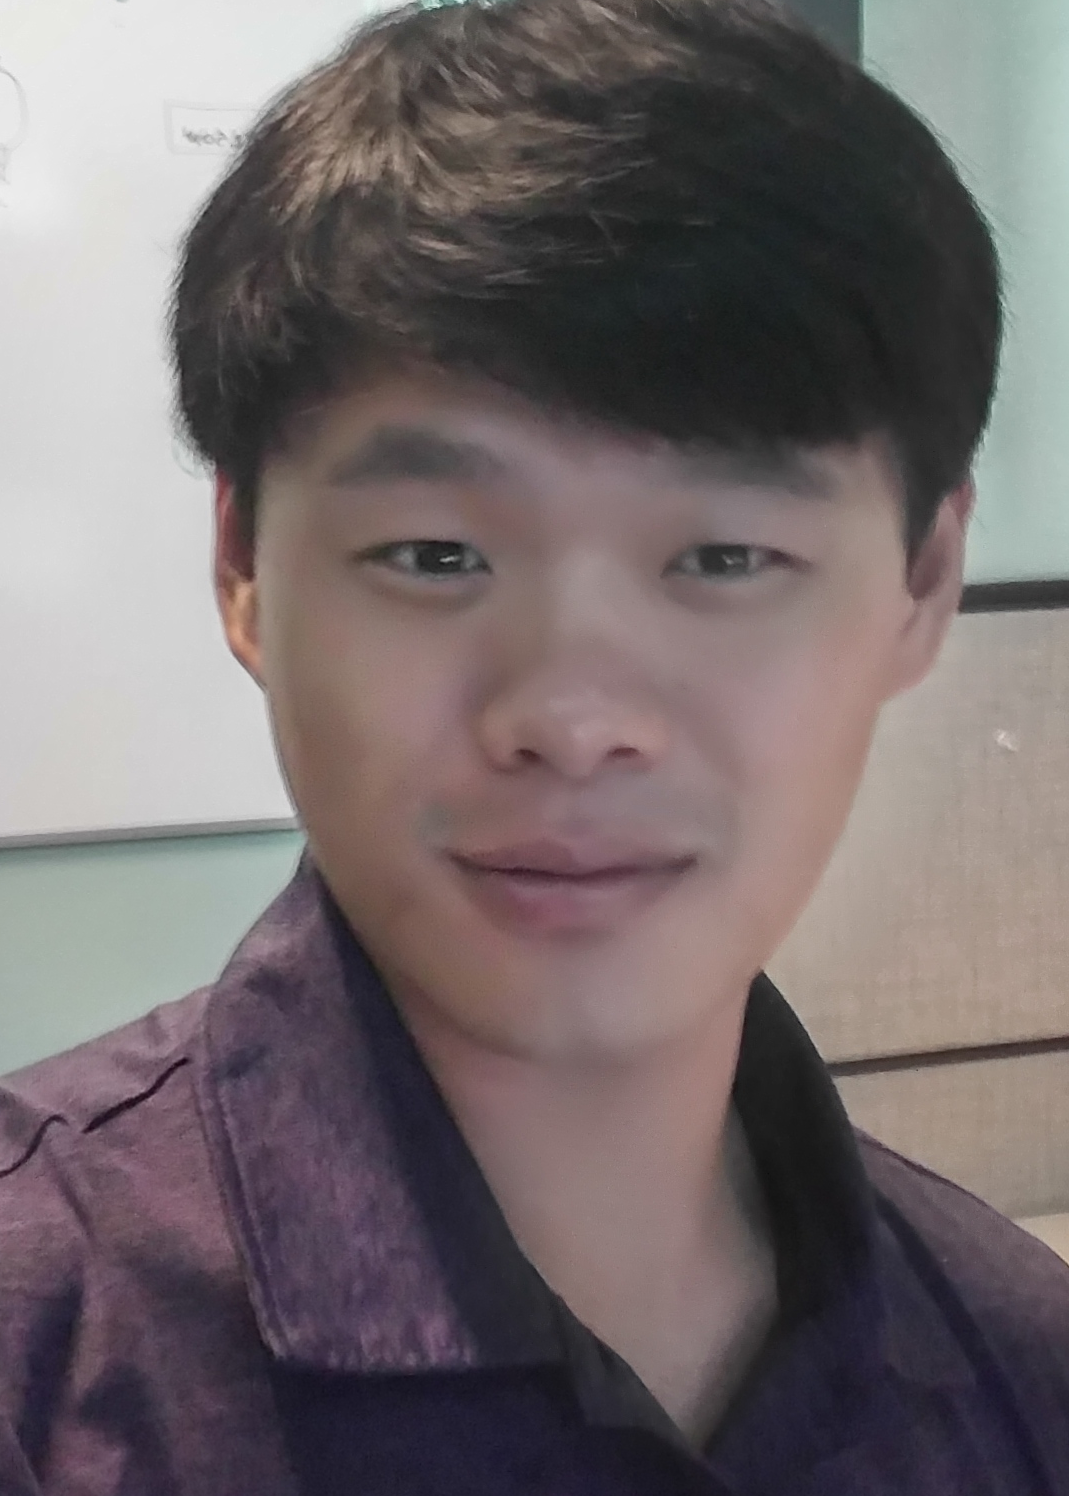
\includegraphics[scale=0.1]{img/Selfie.png}
	~
	~
	~
	~
	~
	\section{Contact}
	~
	404 314 7825
		{\small Atlanta, GA 30345}
	~
	\href{mailto:max.liao@gmail.com}{\textbf{max.liao@gmail.com}}
	~
	\href{github.com/max-liao}{\textbf{github.com/max-liao}}
	~
	\href{www.linkedin.com/in/liao-max}{\textbf{\scriptsize www.linkedin.com/in/liao-max}}
	~
	\section{\large Work Eligibility \vspace{0.1cm}}
	U.S. Citizen
	% use  \hspace{} or \vspace{} to change bubble size, if needed
	\section{\large Computer Skills \vspace{0.2cm}}
	\smartdiagram[bubble diagram]{
		\textbf{Typescript},
		\textbf{Vue},
		\textbf{Angular},
		\textbf{React},
		\textbf{Python},
		\textbf{Matlab},
		\textbf{C/C++},
		\textbf{Eagle},
		\textbf{CAD},
		\textbf{SQL},
		\textbf{RxJS}
	}
	\section{\large Technical Skills \vspace{0.1cm}}
	\textbf{App Development}
	\textbf{UX/UI Design}
	\textbf{Unit Testing}
	\textbf{End to End Testing}
	\textbf{Embedded Systems}
	\textbf{Micro controllers}
	\textbf{CAD Design}
	\textbf{PCB Design}
	\textbf{3D Printing}
	\textbf{Technical Writing}
	\textbf{PID Controllers}
	\textbf{Lab Experience}
	\textbf{Organic Chemistry}
	~
	\section{OS Preference \vspace{0.1cm}}
	\textbf{Linux}
\includegraphics[scale=0.40]{img/5stars.png}
	\textbf{Windows}
\includegraphics[scale=0.40]{img/4stars.png}
	\textbf{iOS}
\includegraphics[scale=0.40]{img/3stars.png}
	~
	\section{Languages \vspace{0.1cm}}
	\textbf{English}
\includegraphics[scale=0.40]{img/5stars.png}
	\textbf{Mandarin}
\includegraphics[scale=0.40]{img/4stars.png}
	\textbf{French}
\includegraphics[scale=0.40]{img/3stars.png}
	\textbf{Spanish}
\includegraphics[scale=0.40]{img/2stars.png}
	~
\end{aside}

\begin{body}
	\section{\vspace{0.05cm} Highlights}
	\begin{itemize}
		\item {Fullstack software engineer with focus on frontend UX web design}
		\item {Software development for elevator dispatch touchscreen devices for TKE}
		\item {C\# app development ATM components for NCR}
		\item {Embedded systems and software development experience in multiple applications \vspace{0.05cm}}
	\end{itemize}
	\section{Experience}
	\begin{entrylist}
		\entry
		{03/19 - now}
		{Software Engineer}
		{TKE}
		{Software development, testing, and support for touchscreen elevator dispatch system including including lobby elevator kiosks, car operating panels, and smart mirrors deployed inside the elevator
			\begin{itemize}
				\item {Developed web app to communicate with devices on job sites}
				\item {App controlled touchscreen displays, settings, content, and software updates originally in AngularJS before upgrade to modern Angular}
				\item {Created ElectronJS app using Vue to simulate destination dispatch of elevators using RS-485 and UDP}
				\item {Added Cypress automated end-to-end testing to codebase}
			\end{itemize}
		}
		\entry
		{11/18 - 6/19}
		{Teacher's Assistant}
		{Georgia Institute of Technology}
		{Full Stack Flex Web Development - teacher's assistant with Trilogy Education\\
			Taught night classes for Georgia Tech Professional Education\\
			Material included NodeJS, ExpressJS, SQL/MongoDB, React}
		\entry
		{4/18 - 12/18}
		{Software Engineer}
		{NCR Corporation}
		{Software and firmware support for the ATM hardware division at NCR \\
			Created and supported analysis tool for the Scalable Deposit Module 2}
		\entry
		{8/15 - 12/17}
		{Research Assistant}
		{Skidaway Institute of Oceanography}
		{Researched UV-wet chemical oxidation dissolved organic carbon (DOC) analyzer for aqueous samples to obtain higher precision, faster speeds, and more adaptable usage than commercial instruments
			% 			\begin{itemize}
			% 				\item Quantitatively measures changes in DOC with a sub-uM target precision two orders of magnitude greater than current commercial devices
			% 				\item Device is more easily transportable, provides faster analysis, and removes system dependency on blank evaluations
			% 				\item Optimized with goal of automated and shipboard analyses of DOC for fresh and salt water\end{itemize}
		}
		\entry
		{4/15 - 9/15}
		{Electrical Engineer}
		{PhytoSynthetix}
		{Made improvements to a fluorometer for grow chamber monitoring at the University of Georgia horticultural greenhouse}
		\entry
		{1/13 - 1/15}
		{Software Test Engineer}
		{Cisco Systems}
		{Install and maintain a continuous integration test framework for set top boxes
			\begin{itemize}
				\item {Developed test software and procedures in Python and C}
				\item {Generated specification and prototype test equipment per product test and repair requirements}
			\end{itemize}
		}
	\end{entrylist}
	\section{ \vspace{-0.1cm} Education \vspace{0.1cm} }
	\par
	\begin{entrylist}
		\entry
		{2015 - 2017}
		{Master of Science in Biological Engineering}
		{University of Georgia}
		{Research Assistant at Skidaway Institute of Oceanography
			\begin{description}
				\item {Advisers: Dr. Aron Stubbins and Dr. Mark Haidekker}
				\item {Certificate in Coastal and Oceanographic Engineering}
			\end{description}}
		\entry
		{2008 - 2012}
		{Bachelor of Science in Electrical Engineering}
		{Georgia Institute of Technology}
		{
			Undergraduate Research Opportunities Program - a multiple antenna energy harvesting circuit involving frequency selective surfaces
			\begin{description}
				\item {Adviser: Dr. Manos Tentzeris}
			\end{description}
		}
		\entry
		{2018}
		{Full Stack Flex Web Development}
		{Georgia Institute of Technology}
		{Georgia Tech Professional Education coding bootcamp}
	\end{entrylist}
\end{body}
\end{document}

% \newpage
% 	\section{Certifications\\}
%     	\begin{entrylist}
%     		\entry
%     		{08/2018}
%     		{Full Stack Flex Web Development}
%     		{Georgia Institute of Technology}
%     		{Professional education certificate for a full stack web development coding bootcamp}
%     		\entry
%     		{12/2017}
%     		{Coastal and Oceanographic Engineering}
%     		{University of Georgia}
%     		{Graduate certificate for multi-disciplinary program in engineering and marine sciences emphasizing marine instrumentation and numerical modeling of near-shore and coastal processes\\ Includes course work in engineering and marine sciences as well as a research and design component at the graduate level}
%     	\end{entrylist}
% % 	\section{Other Info}
% %     	~
% %     	Can read/write French and Spanish\\
% %     	\emph{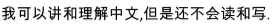
\includegraphics[scale=1]{img/Chinese.PNG}}\\
% % 	\section{Publications}
% %     	Max Liao\\ \textbf{A Precision UV-Wet Chemical Oxidation Dissolved Organic Carbon Analyzer}\\
% %     	MS Thesis. University of Georgia, 2017
% %     	\\\\
% %     	Wenting Gu, Peng Cheng, Arindam Ghosh, Max Liao, Boxiong Liao, Ali Beskok, Zhili Hao\\
% %     	\textbf{Detection of distributed static and dynamic loads with electrolyte enabled distributed transducers in a polymer based microfluidic device}\\
% %     	\emph{ Journal of Micromechanics and Microengineering, Vol. 23, March 2013, 035015 (15pp), doi:10.1088/09601317/23/3/035015 (featured in IOPselect) }
% %     	\\\\
% %     	Wenting Gu, Peng Cheng, Arindam Ghosh, Max Liao, Boxiong Liao, Ali Beskok, Zhili Hao\\
% %     	\textbf{A polymer based microfluidic resistive sensor for detecting distributed loads}\\
% %     	\emph{ ASME International Mechanical Engineering Congress and Exposition (IMECE2012), \\ Nov. 9-15, 2012, Houston, Texas, IMECE201287672 (Best Paper Award in the MEMS Division) }
% %     	\\
% %     	\begin{flushleft}
% %     	\end{flushleft}
%     	\begin{flushright}
%     		\emph{Max Liao }
%     		\emph{Software Engineer}
%     	\end{flushright}
% \end{body}
% \begin{aside}
% ~
% 	~
% 	~
% 	\section{Languages}
% 	~
% 	\textbf{English}
\includegraphics[scale=0.40]{img/5stars.png}
% 	\textbf{Mandarin}
\includegraphics[scale=0.40]{img/4stars.png}
% 	\textbf{French}
\includegraphics[scale=0.40]{img/3stars.png}
% 	\textbf{Spanish}
\includegraphics[scale=0.40]{img/2stars.png}
% 	~
% \end{aside}
% \end{document}